% Source: Code/ML_overlay/ir_rgb_registration/paper/ml_overlay_report_materials/ir_rgb_registration_report/figures/fig_deformable_conv.tex
\documentclass[tikz,border=10pt]{standalone}
\usepackage{tikz}
\usetikzlibrary{arrows.meta,positioning,calc}

\definecolor{garnet}{RGB}{115,0,10}
\definecolor{rose}{RGB}{204,46,64}
\definecolor{atlantic}{RGB}{70,106,159}
\definecolor{congaree}{RGB}{31,65,77}
\definecolor{black90}{RGB}{54,54,54}
\definecolor{black50}{RGB}{162,162,162}

\begin{document}
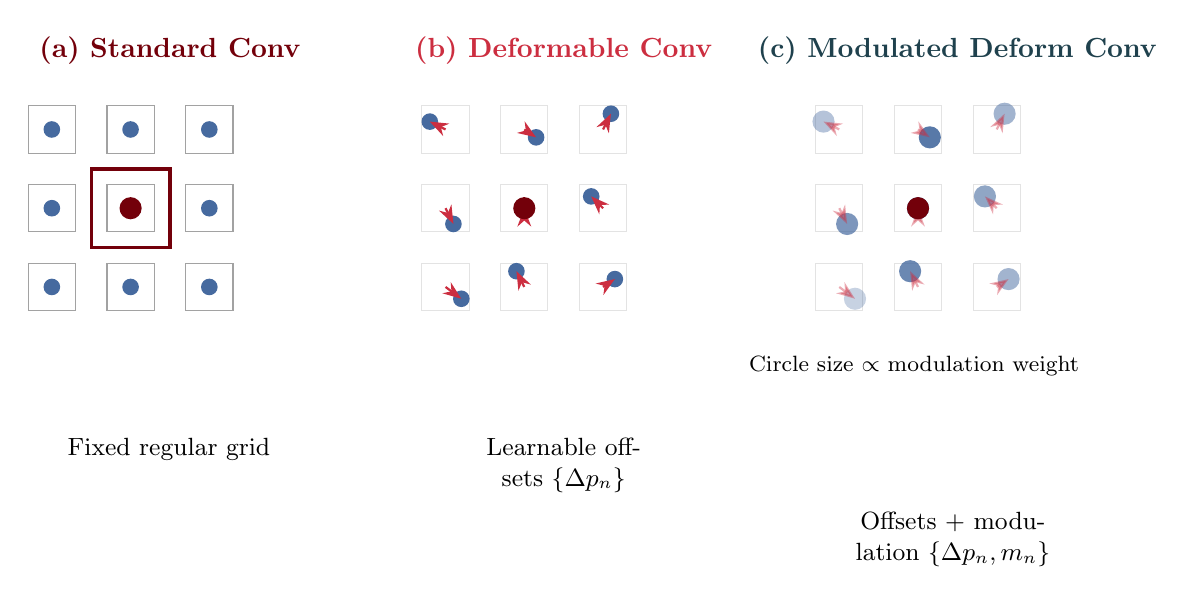
\begin{tikzpicture}[>=Stealth]

    % (a) Standard 3x3 convolution
    \begin{scope}[local bounding box=standard]
        \node[font=\bfseries, garnet] at (1.5,3) {(a) Standard Conv};

        % Grid
        \foreach \x in {0,1,2} {
            \foreach \y in {0,1,2} {
                \fill[atlantic] (\x,\y) circle (3pt);
                \draw[black50, thin] (\x-0.3,\y-0.3) rectangle (\x+0.3,\y+0.3);
            }
        }

        % Center point
        \fill[garnet] (1,1) circle (4pt);
        \draw[garnet, very thick] (0.5,0.5) rectangle (1.5,1.5);
    \end{scope}

    % (b) Deformable convolution
    \begin{scope}[shift={(5,0)}, local bounding box=deformable]
        \node[font=\bfseries, rose] at (1.5,3) {(b) Deformable Conv};

        % Regular grid positions (light)
        \foreach \x in {0,1,2} {
            \foreach \y in {0,1,2} {
                \draw[black50, thin, opacity=0.3] (\x-0.3,\y-0.3) rectangle (\x+0.3,\y+0.3);
            }
        }

        % Deformed sample points with offsets
        \coordinate (c) at (1,1);
        \foreach \x/\y/\dx/\dy in {0/0/0.2/-0.15, 1/0/-0.1/0.2, 2/0/0.15/0.1,
                                     0/1/0.1/-0.2, 1/1/0/0, 2/1/-0.15/0.15,
                                     0/2/-0.2/0.1, 1/2/0.15/-0.1, 2/2/0.1/0.2} {
            \fill[atlantic] (\x+\dx,\y+\dy) circle (3pt);
            \draw[->, rose, thick] (\x,\y) -- (\x+\dx,\y+\dy);
        }

        % Center point
        \fill[garnet] (1,1) circle (4pt);
    \end{scope}

    % (c) Modulated deformable convolution
    \begin{scope}[shift={(10,0)}, local bounding box=modulated]
        \node[font=\bfseries, congaree] at (1.5,3) {(c) Modulated Deform Conv};

        % Regular grid positions (light)
        \foreach \x in {0,1,2} {
            \foreach \y in {0,1,2} {
                \draw[black50, thin, opacity=0.3] (\x-0.3,\y-0.3) rectangle (\x+0.3,\y+0.3);
            }
        }

        % Deformed sample points with varying opacity (modulation)
        \foreach \x/\y/\dx/\dy/\m in {0/0/0.2/-0.15/0.3, 1/0/-0.1/0.2/0.8, 2/0/0.15/0.1/0.5,
                                       0/1/0.1/-0.2/0.7, 1/1/0/0/1.0, 2/1/-0.15/0.15/0.6,
                                       0/2/-0.2/0.1/0.4, 1/2/0.15/-0.1/0.9, 2/2/0.1/0.2/0.5} {
            \fill[atlantic, opacity=\m] (\x+\dx,\y+\dy) circle (4pt);
            \draw[->, rose, thick, opacity=0.4] (\x,\y) -- (\x+\dx,\y+\dy);
        }

        % Center point
        \fill[garnet] (1,1) circle (4pt);

        % Modulation legend
        \node[font=\footnotesize, align=center] at (1,-1) {
            Circle size $\propto$ modulation weight
        };
    \end{scope}

    % Annotations
    \node[below=1.5cm of standard, font=\small, text width=3cm, align=center] {
        Fixed regular grid
    };
    \node[below=1.5cm of deformable, font=\small, text width=3cm, align=center] {
        Learnable offsets $\{\Delta p_n\}$
    };
    \node[below=1.5cm of modulated, font=\small, text width=3cm, align=center] {
        Offsets + modulation $\{\Delta p_n, m_n\}$
    };

\end{tikzpicture}
\end{document}
